\documentclass{llncs}



\usepackage{amsmath,amsfonts}
\usepackage{xspace}
\usepackage{txfonts}
\usepackage{proof}

\usepackage{pgf}
\usepackage{tikz}
\usetikzlibrary{arrows,automata}
\usetikzlibrary{positioning}
\usetikzlibrary{shapes}

\usepackage{xspace}

\newcommand{\eg}{\textit{e.g.}}
\newcommand{\etc}{\textit{etc.}}
\newcommand{\ie}{\textit{i.e.}}
\newcommand{\cf}{\textit{cf.}}
\newcommand{\lb}{\texttt{\char'173}} \newcommand{\rb}{\texttt{\char'175}} \newcommand{\wrt}{wrt.\xspace}

\newcommand{\secref}[1]{Sec.~\ref{#1}}
\newcommand{\CTLs}{\ensuremath{\text{CTL}^\ast}\xspace}
\newcommand{\CTLsFO}{\ensuremath{\text{CTL}^\ast(\text{FO})}\xspace}

\newcommand{\calC}{{\cal C}}
\newcommand{\calD}{{\cal D}}
\newcommand{\calF}{{\cal F}}
\newcommand{\calP}{{\cal P}}
\newcommand{\calT}{{\cal T}}
\newcommand{\calS}{{\cal S}}
\newcommand{\calI}{{\cal I}}

\newcommand{\Form}{\mathsf{Form}}
\newcommand{\Guard}{\mathsf{Guard}}
\newcommand{\GProg}{\mathsf{GProg}}
\newcommand{\Update}{\mathsf{Update}}
\newcommand{\db}{\ensuremath{\mathit{db}}\xspace}
\newcommand{\DB}{\ensuremath{\mathit{DB}}\xspace}
\newcommand{\sfdb}{\ensuremath{\mathsf{db}}\xspace}
\newcommand{\sftrue}{\ensuremath{\mathsf{true}}\xspace}
\newcommand{\sffalse}{\ensuremath{\mathsf{false}}\xspace}
\newcommand{\entry}{\ensuremath{\mathrm{entry}}\xspace}
\newcommand{\exit}{\ensuremath{\mathrm{exit}}\xspace}
\newcommand{\init}{\ensuremath{\mathrm{init}}\xspace}
\newcommand{\final}{\ensuremath{\mathrm{final}}\xspace}

\newcommand{\pqE}{\mathsf{E}}
\newcommand{\pqA}{\mathsf{A}}

\newcommand{\toU}{\mathsf{U}}
\newcommand{\toR}{\mathsf{R}}
\newcommand{\toX}{\mathsf{X}}
\newcommand{\toF}{\mathsf{F}}
\newcommand{\toG}{\mathsf{G}}
\newcommand{\toWX}{\mathsf{\overline{X}}}
\newcommand{\toWU}{\mathsf{W}}

\newcommand{\ltlU}{\toU}
\newcommand{\ltlX}{\toX}
\newcommand{\ltlF}{\toF}
\newcommand{\ltlG}{\toG}
\newcommand{\ltlWX}{\toWX}
\newcommand{\ltlWU}{\toWU}
\newcommand{\ltlR}{\toR}


\newcommand{\KW}[1]{\mathsf{#1}}

\def\void{}
\newcommand{\infrule}[3][\void]{{\renewcommand\arraystretch{1.25}
    \ifx\void#1\else\IR{#1}\hspace{0.5em}\fi
    \begin{array}[c]{@{\hspace*{1em}}c@{\hspace*{1em}}}#2\\\hline #3
    \end{array}}}

\newcommand{\IR}[1]{\text{\textsf{#1}}\xspace}



 


\ifnum\pdfoutput>0
\synctex=1 \else
\usepackage[active]{srcltx} \fi

\pagestyle{plain}

\begin{document}
\setlength\abovedisplayskip{5pt plus 2pt minus 4pt}
\setlength\belowdisplayskip{5pt plus 2pt minus 4pt}

\title{Reasoning with Data-Centric Business Processes}

\author{Andreas Bauer \and Peter Baumgartner \and Michael Norrish}
\institute{NICTA\thanks{\scriptsize NICTA is funded by the Australian Government as
    represented by the Department of Broadband, Communications and the
     Digital Economy and the Australian Research Council through the ICT
     Centre of Excellence program.} Software Systems Research Group,
  and\\The Australian National University}

\maketitle

\pagestyle{plain}



\begin{abstract}
We describe an approach to modelling and reasoning about data-centric business processes and present a form of general model checking.
Our technique extends existing approaches, which explore systems only from concrete initial states.

Specifically, we model business processes in terms of smaller fragments, whose possible interactions are constrained by first-order logic formulae.
In turn, process fragments are connected graphs annotated with instructions to modify data.
Correctness properties concerning the evolution of data with respect to processes can be stated in a first-order branching-time logic over built-in theories, such as linear integer arithmetic, records and arrays.

Solving general model checking problems over this logic is considerably harder than model checking when a concrete initial state is given.
To this end, we present a tableau procedure that reduces these model checking problems to first-order logic over arithmetic. The resulting proof obligations are passed on to appropriate ``off-the-shelf'' theorem provers.
We also detail our modelling approach, describe the reasoning components and report on first experiments.

\end{abstract}



\section{Introduction}
Data is becoming increasingly important to large organisations, both private enterprises and large government departments.
Recent headlines on ``big data'' (\cf~\cite{NYT120212}) suggest that many organisations manage unprecedented amounts of structured data, and that worldwide, the volume of information processed by machines and humans doubles approximately every two years.
Organisations need to be able to organise and process data according to their defined business processes, and according to business rules that may further specify properties of the processed data.

Unfortunately, most approaches to business process modelling do not adequately support the analysis of the complex interactions and dependencies that exist between an organisation's processes and data.
Although they may support process analysis, helping users find and remove errors in their models, most fall short when the processes are closely tied to structured data.
The reasons for this are specific to the concrete formalism used for the analyses, but can normally be traced back to the fact that classical propositional logic or discrete Petri-nets are used.
Neither of these can adequately represent structured data and the operations on it.
In other words, these tools' analyses make coarse abstractions of the data, and instead focus mostly on the correctness of workflows.

The business artifact approach, initially outlined in \cite{DBLP:journals/ibmsj/NigamC03}, was one of the first to tackle this issue.
It systematically elevates data to be a ``first-class citizen'', while still offering automated support for process analysis.
Its cornerstones are
\emph{artifacts}, which are records of data values that can change over
time due to the modifications performed by \emph{services}, which are
formalised using first-order logic.
Process analysis is provided, essentially, by means of model checking.
That is, the following question is answered automatically: given some artifact model, a database providing initial values, and a correctness property in terms of a first-order linear-time temporal logic formula (called LTL-FO), do all possible artifact changes over time satisfy the correctness property?
For the constraints given in~\cite{DBLP:conf/bpm/DamaggioDHV11}, this problem is always decidable.

In this paper, we present an approach to modelling and reasoning about data-centric business processes, which is similar to this work, but which offers reasoning support that goes beyond that work's ``concrete model checking''.
Our approach is based on \emph{process fragments} that describe specific tasks of a larger process, as well as \emph{constraints} for limiting the interactions between the fragments.
As such it is also inspired by what is known as \emph{declarative
  business process modelling}~\cite{DBLP:conf/bpm/PesicA06}, meaning
that users do not have to create a single, large transition system
containing all possible task interleavings.
Instead, users can create many small process fragments whose interconnections are governed by rules that determine which executions are permitted.

In our framework, those rules are given by first-order temporal logic.
Unlike~\cite{DBLP:conf/bpm/DamaggioDHV11}, we choose to extend \CTLs, \ie, a branching time logic, rather than LTL, since process fragments are essentially annotated graphs and \CTLs is, arguably, an appropriate formalism to express its properties (\cf~\cite{clarke_em-etal:1999a}).
Our database is given in terms of JSON objects~\cite{JSON}, enriched by a custom, static type system which models and preserves the type information of any input data.
Process fragments may modify data, and one can easily state and answer the concrete model checking problem as outlined above.

However, our approach also works if
one does not start with an initial concrete database; that is, we intend to not only check
whether it is possible to, reach a bad state (\eg, a set of data for
which no process fragment is applicable) from some given state (\ie,
the initial set of data), but also to determine whether for \emph{any}
set of data a bad state can be reached.
In other words, we support what we call \emph{generic model checking}.
As the domains of many data items are infinite (\eg, any item of type integer), this problem is considerably harder, in fact, generally undecidable.

Informally, the two reasoning problems we are interested in are:
\begin{description}
\item[Concrete data model checking problem:] Given a specification , a
  database , and a \CTLsFO  formula . Does
   hold?
\item[Unrestricted model checking problem:] Given a specification  and
  a \CTLsFO  formula . For every database , does  hold?
\end{description}
As will become clear below, a \emph{specification} is comprised of a process model,
logical definitions, and constraints to combine process fragments. The relation 
 means that the pair  satisfies the query .
See Section~\ref{sec:process} for the precise semantics.

Without any further restrictions, both problems are not even semi-decidable.  This
can be seen, \eg, by reduction from the domain-emptyness problem of 2-register
machines. Hence, practical approaches need to work with restrictions to recover more
pleasant complexity properties.



The rest of the paper is structured as follows.
In Section~\ref{sec:example} we present a running example.
In Section~\ref{sec:data} we explain the way we handle the rich data of our models: with JSON values, a special type system for those values, and a sorted first order logic for further constraining and describing those values.
This much covers business \emph{rules}; in Section~\ref{sec:process}, we describe how we can model \emph{processes}.
When processes (actually process \emph{fragments}) combine with rules, we get what we call \emph{specifications}.
In Section~\ref{sec:ctlsfo-tableaux}, we describe the tableau-based model checking algorithm that is used to decide user queries of the two sorts identified above.
Section~\ref{sec:experiments} discusses how we have implemented our technology, and describes some experimental results.
Finally, we conclude in Section~\ref{sec:conclusion}.








\section{A Running Example: Purchase Order}
\label{sec:example}

\begin{figure}[tbp]
\textbf{Process model:}\\
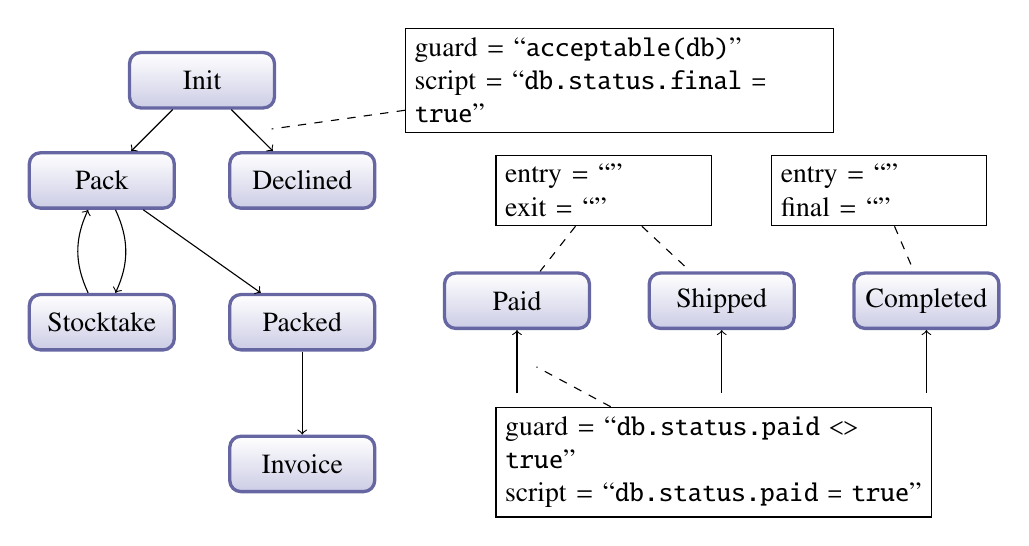
\begin{tikzpicture}
  [
   node distance=1.8cm,
   state/.style={
     text width=1.7cm, rectangle, rounded corners, draw=black,
     very thick, minimum height=2em, inner sep=2pt, text centered},
   task/.style={
     rectangle, rounded corners, shade, top color=white,
     bottom color=blue!50!black!20, draw=blue!40!black!60,
     very thick}
  ]



 \node[state,task]                      (INIT)      { Init };
 \node[state,task,below left of=INIT]   (PACK)      { Pack };
 \node[state,task,below of=PACK]        (STOCKTAKE) { Stocktake };
 \node[state,task,below right of=INIT]  (DECLINED)  { Declined };
 \node[state,task,below of=DECLINED]    (PACKED)    { Packed };
 \node[state,task,below of=PACKED]      (INVOICED)  { Invoice };

 \path[->] (INIT) edge                    node[left]  {} (PACK);
 \path[->] (INIT) edge                    node[right](DECLINED_EDGE) {} (DECLINED);
 \path[->] (PACK) edge[bend left=25]      node[right] {} (STOCKTAKE);
 \path[->] (STOCKTAKE) edge[bend left=25] node[left]  {} (PACK);
 \path[->] (PACK) edge                    node[right] {} (PACKED);
 \path[->] (PACKED) edge                  node[right] {} (INVOICED);



 \node[state, task, right of=INIT, yshift=-2.8cm,xshift=2.2cm] (PAID)      { Paid };
 \node[below of=PAID,yshift=0.5cm]                             (PAID_INCOMING) { };
 \path[->] (PAID_INCOMING) edge node[right](PAID_EDGE) {} (PAID);

 \node[state, task, right of=PAID,xshift=0.8cm]        (SHIPPED)   { Shipped };
 \node[below of=SHIPPED,yshift=0.5cm]                  (SHIPPED_INCOMING) { };
 \path[->] (SHIPPED_INCOMING) edge node[right] {} (SHIPPED);

 \node[state, task, right of=SHIPPED,xshift=0.8cm]       (COMPLETED) { Completed };
 \node[below of=COMPLETED,yshift=0.5cm]                  (COMPLETED_INCOMING) { };
 \path[->] (COMPLETED_INCOMING) edge node[right] {} (COMPLETED);



 \node[above of=PAID,yshift=-0.4cm,xshift=1.1cm,rectangle split parts=5,
       draw,text width=2.5cm] (LEGEND_PAID)
       {
         entry = ``''\\
         exit = ``''
       };
 \draw[dashed] (LEGEND_PAID) -- (PAID);
 \draw[dashed] (LEGEND_PAID) -- (SHIPPED);

 \node[below of=PAID,yshift=-0.25cm,xshift=2.5cm,rectangle split parts=5,
       draw,text width=5.3cm] (LEGEND_PAID_EDGE)
       {
guard = ``\texttt{db.status.paid <> true}''\\
         script = ``\texttt{db.status.paid = true}''
};
 \draw[dashed] (LEGEND_PAID_EDGE) -- (PAID_EDGE);

 \node[above of=COMPLETED,yshift=-0.4cm,xshift=-0.6cm,rectangle split parts=5,
       draw,text width=2.5cm] (LEGEND_COMPLETED)
       {
         entry = ``''\\
         final = ``''
       };
 \draw[dashed] (LEGEND_COMPLETED) -- (COMPLETED);

 \node[right of=INIT,yshift=0cm,xshift=3.5cm,rectangle split parts=3,
       draw,text width=5.2cm] (LEGEND_DECLINED)
       {
         guard = ``\texttt{acceptable(db)}'' \\
         script = ``\texttt{db.status.final = true}''
};
 \draw[dashed] (LEGEND_DECLINED) -- (DECLINED_EDGE);
\end{tikzpicture}

\textbf{Definitions:}

completed: 

accepted: 

readyToShip:  \ldots\\

\textbf{Constraints:}

nongold: 

\caption{Model of a purchase order system as process fragments and definitions.}
\label{fig:purchase}
\end{figure}

In this section, we introduce a simplified model of a purchase order
system using process fragments.  The purpose of the modelled system is
to accept incoming purchase orders and process them further (packing,
shipping, etc.), or to decline them straight away if there are
problems.
The whole model is depicted as a graph in Fig.~\ref{fig:purchase}, where
the biggest process fragment is on the left, with further atomic
fragments beside it (labelled Paid, Shipped, and Completed,
respectively).
Both process tasks, represented as nodes in the graph,
and connections are typically annotated with extra information.
Node annotations determine whether or not a node is an initial and/or a final node, an entry and/or an exit node.
This information is used to constrain the ways in fragments can connect.
Edges can carry a guard given as a
formula and a simple program written in the programming language Groovy.
The purpose of the program (given in the field ``script'') is to modify
the underlying database, which is referred to by the variable \verb+db+.

The depicted system model has one initial node, Init, where it
waits for a purchase order to arrive.
Then, the system can either start to pack (\ie, enter node Pack), or decline the order (\ie, enter node
Declined).
An order can be declined if the guard () in the annotation of edge  is satisfied.
The predicate  is defined in the
Definitions section of our input specification.
In a nutshell, the sections Definitions and Constraints contain domain-knowledge, encoded as logical rules.
(The constraint named ``nongold'' states that non-gold customers
must pay before shipment;  is the ``weak until'' operator.)

If the order is not declined, an attempt will be made to pack its constituents.
If all are in stock, the process will continue to the node Packed.
However, if one or more items are missing, they need to be ordered in, which is expressed in the loop between the nodes Pack and Stocktake.

Informally, process fragments are linked together as follows.
Starting from a state comprised of an \init node and a given initial database, an outgoing transition from the current state can only be executed
if it satisfies the transition's guard.
If it is satisfied, the associated program is executed to determine the new value of the database, and the edge's target node becomes the new current state.
The \entry and \exit annotations impose implicit constraints on how
fragments can be combined: the execution of a new process fragment must
always start with its \entry node\footnote{For simplicity we assume
  every fragment contains exactly one entry node.} coming from an \exit node. In
other words, there are implicit transitions between all \exit and all \entry nodes. 
However, if a guard is associated to an
\entry \emph{node}, this guard sits on all its implicit incoming transitions. 
The computation stops if from the current
state no successor can be reached, either because there is no outgoing
edge, the guards of all outgoing edges are not satisfied by the
current state, or a depth limit has been reached.

In our example, two possible sequences are Init  Declined, or
Init  Pack  \ldots  Invoice
 Paid  Shipped Completed.
It is not required to cover all fragments, as illustrated by the first run.

The database which can be modified by the programs given in the
``script'' annotations, is represented as a JSON object.  See, for
example, left hand side of Fig.~\ref{fig:data}.  (The right hand side
contains type definitions for the JSON data, see also
\secref{sec:data}.)  The program annotated on
edge , which leads into node Declined, simply sets the field
\texttt{final} inside \texttt{status} to \texttt{true}.
Crucial for our example is the list of open items, under
\texttt{status}, which has to be empty to be able to ship a purchase
order.  If it is not, constituents of the order are missing and need to
be ordered until the list is empty.

As for sample queries consider the \CTLsFO formula
, which can be seen as a \emph{planning} goal.
The runs on the model above that \emph{falsify} it lead to a database  that has reached a ``final'' state, with  being set to .
Planning queries are useful, \eg, for flexible
process configuration from fragments during runtime. Another interesting query is
.
It is a safety property, saying that at all stages in the process run, and for all possible stock items, the number of available items is non-negative.
Such queries are typical during design time, and pose an unrestricted model checking problem.



\begin{figure}[tbp]
\begin{minipage}[t]{0.5\linewidth}
\begingroup
\fontsize{7pt}{9pt}\selectfont
\begin{verbatim}
{   "order" : [1],
    "gold"  : true,
    "stock" : [ { "ident" : "Mouse",
                  "price" : 10,
                  "available" : 0  },
                { "ident" : "Monitor",
                  "price" : 200,
                  "available" : 2  },
                { "ident" : "Computer",
                  "price" : 1000,
                  "available" : 4  } ],
    "status" : {  "open" : [],
                  "value" : 0,
                  "shipping" : 0,
                  "paid" : false,
                  "shipped" : false,
                  "final" : false }    }
\end{verbatim}
\endgroup
\end{minipage}
\begin{minipage}[t]{0.5\linewidth}
\begingroup
\fontsize{7pt}{9pt}\selectfont
\begin{verbatim}
   DB  = { order: List[Integer],
           gold: Bool,
           stock: List[Stock],
           status: Status      }

 Stock = { ident: String,
           price: Integer,
           available: Integer  }

Status = { open: List[Integer],
           value: Integer,
           shipping: Integer,
           paid: Bool,
           shipped: Bool,
           final: Bool         }
\end{verbatim}
\endgroup
\end{minipage}
\caption{\emph{Left:} Example database as JSON document. \emph{Right:} JSON type constraints.}
\label{fig:data}
\end{figure}




\section{Modelling Data With JSON Logic}
\label{sec:data}
Faithful modelling of business processes requires being able to model the objects (or \emph{data}) manipulated by the processes and, of course, their evolution over time.
In this section we focus on data modelling, which is based on JSON extended with a type system.

JSON~\cite{JSON} is simple, standardised, textual data representation format.  In
addition to a standard set of atomic values such as integers and strings, JSON
supports two structuring techniques: sequencing (``arrays'') and arbitrarily nested
hierarchies (through ``objects'').
Our choice of JSON (rather than XML, say), is based on the ease with which it can be
written and understood by humans.  JSON is sufficiently rich to be a plausible format
for representing the data used in business processes, and its human ease-of-use is
extremely helpful. 

Other than simply being the medium in which data is represented, there are two
important functions that JSON must support.  Firstly, it must be possible to
manipulate JSON values in the course of executing a specification. This
functionality is realised through the use of the Groovy programming notation.

Secondly, it must be possible to express \emph{logical} predicates over JSON values,
both to guard process transitions and to pick out certain forms of value that are of
interest.  In particular, if a specification is to achieve a particular end-goal,
with a database being in a particular configuration, we need to be able to describe
how the various values in that database inter-relate.  It is this that motivates our
choice of the logically expressive capabilities of first order logic, together with
sorts such as lists and numbers.

In addition to first-order predicates, we also use a simple type system over JSON
values.  This provides a simple mapping into the sorts of our underlying first-order logic.
We note that the type system is indispensable for unrestricted model checking, in
order to derive from it logical axioms for object and array manipulations.

\subsection{A Type System for JSON}
First we briefly summarise the syntax that is fully described in the IETF~RFC~\cite{JSON}:
JSON values can be numbers, booleans (\texttt{true} and \texttt{false}), strings (written between double-quotes, \eg, \texttt{"a~string"}) and a special value \texttt{null}.
JSON's \emph{arrays} are written as comma-separated values between square-brackets, \eg, \texttt{[1,~"string",~[true]]}.
JSON \emph{objects} are similar to records or structures in languages such as Pascal and C.
They are written as lists of field-name/value pairs between braces.
Both forms are illustrated in Figure~\ref{fig:data}.

\newcommand{\obj}[1]{\texttt{Obj}\lb#1\rb}
Sibling field-names within an object should be unique, and are considered unordered.
Therefore, an object can be thought of as a finite map from field-names to further JSON values.
Following this conception, we write \obj{} to denote an object whose field names are the domain of finite map , with field 's value being .


\newcommand{\intty}{\texttt{Integer}}
\newcommand{\boolty}{\texttt{Bool}}
\newcommand{\stringty}{\texttt{String}}
\newcommand{\listtyopname}{\texttt{List}}
\newcommand{\listty}[1]{\listtyopname[#1]}
\newcommand{\optiontyopname}{\texttt{Option}}
\newcommand{\optionty}[1]{\optiontyopname[#1]}
\newcommand{\objtyopname}{\texttt{ObjTy}}
\newcommand{\objty}[1]{\objtyopname\lb#1\rb}
\newcommand{\enumtyopname}{\texttt{EnumTy}}
\newcommand{\enumty}[1]{\enumtyopname[#1]}
\newcommand{\dom}{\mathrm{dom}}

JSON does not impose any restrictions on the structure of values.  For example, a
list may contain both strings and integers.  However, we choose to restrict this
freedom with a simple type system comparable to those in third-generation languages
such as C.  Let JSON types be denoted by , ,  \etc, then
{\small

}
where  is a finite map from strings to types, and  is a list of strings.

The \optiontyopname{} and \enumtyopname{} types are the only ones that do not have a obvious connection back to a set of JSON values.
The \optiontyopname{} type is used to allow for values that are not necessarily always initialised, but which come to acquire values as a process progresses.
We do not expect to see the option-constructor occur with multiple nestings, \eg, a type such as .
The \enumtyopname{} type is used to model finite enumerated types, where each value is represented by one of the strings in the provided list.
This flexibility in the type system allows for more natural modeling.

Values are assigned types with the following inductive relation, where we write  to indicate that JSON value  has type , where the meta-variables  and 
correspond to all possible integer and string values respectively, and where we use
 to mean that element  is a member of list :
{\small
3mm]
\infer{s : \enumty{\mathit{sl}}}{s \in \mathit{sl}} \qquad
\infer{\texttt{null} : \optionty{\tau}}{} \qquad
\infer{v : \optionty{\tau}}{v : \tau}
\3mm]
\infer{\obj{\mathit{vf}} : \objty{\mathit{tf}}}{
  \dom(\mathit{vf}) = \dom(\mathit{tf}) &
  \forall s \in \dom(\mathit{vf}). \;\mathit{vf}(s) : \mathit{tf}(s)
}
\end{array}

  N &= \textstyle \bigcup_{1\le i \le k} N_i  &   E &= (\textstyle \bigcup_{1\le i \le k} E_i) \cup E^+ &
  \lambda^\mathsf{E} &= (\textstyle \bigcup_{1\le i \le k} \lambda^\mathsf{E}_i) \cup  \lambda^+

  E^+ &= \{ (m,n) \mid
   m \in  N_i \text{, } n \in  N_j \text {, }
  \exit \in  \lambda^\mathsf{N_i}(m) \text { and }
  \entry \in   \lambda^\mathsf{N_j}(n) \text{, for some } 1 \le i,j \le k \}\
For the above construction to be well-defined we require that every \entry node in
every fragment  is also labeled with a guard  (which could be ).


\subsection{Definitions and Constraints}
Definitions are logical abbreviations. As such, they are not semantically necessary.
Nonetheless, just as in mathematics, they are a crucial aid in the construction and
comprehensibility of useful models. Formally,
a \emph{definition (for )} is a closed formula of the form  where 
is list of variables of sorts ,  is a predicate symbol of the
proper arity, and  is a formula.

Constraints specify how process fragments can be combined. The idea has been pursued
before, \eg, in the Declare system~\cite{DBLP:conf/bpm/PesicA06} which uses \emph{propositional}
(linear) temporal logic for that. In order to take data into account, we work with a
fragment of \CTLs over first-logic, which we refer to as \CTLsFO.
The syntax of our \CTLsFO state formulae is given by

where  is a FO formula with free variables at most , and  a path formula defined via
. (The operator  is ``weak next''.)
A \emph{constraint} then is simply a state formula. Notice that because constraints may
contain the free variable , our logic is \emph{not} obtained from propositional
\CTLs by replacing propositional variables by closed formulas.

Figure~\ref{fig:purchase} contains some examples of definitions and constraints.


\subsection{Specifications and Semantics}
The modelling components describing so far are combined into \emph{specifications}.
Formally, a \emph{specification}  is a tuple  where  is a process,  is a set of definitions and
 is a set of constraints.
An \emph{instance  (of )} is a pair , where 
is a database (as a term) and  is a specification.

We are now in the position to provide a formal definition for the model checking
problems stated in the introduction.
Let  be as above, where 
is of the form  and  a state formula with free variables
at most , the \emph{query}.

As a first step to define the satisfaction relation  between an
instance and a query we make
the constraints  part of the query. Assume  is given in negation
normal form (this is always possible) and that it starts with a path quantifier
( or ). The \emph{expanded query } is the formula
 if , for some formula , and it is
 if .
Here,  is read as a conjunction of its elements. (The rationale for this definition is that the
desired treatments of constraints is indicated by the path quantifier in the query.)
Notice that with  also  is a query.
Now define  iff , \ie,
the triple  \emph{satisfies} .
It remains to define the latter satisfaction relation, which we turn to now.

As a convenience, we say that \emph{ contains a transition }.  if  and , for some
guard  and Groovy program  as an update term.

A \emph{run  (of ) from } is a possibly
infinite sequence  of pairs of nodes and
databases, also called \emph{states}, such that (i)
 contains transitions of the form  , (ii)  and (iii) . In item (i)
in case  the node  is meant to be the initial node  in .
Notice that in item (ii) the definitions  play the role of axioms from which
the instantiated guard  is to follow.
Occasionally the nodes in a run are not important. and we confuse a run with its
projection on the states  .

For a run   and  we define ,
sometimes also .
By  we denote the truncated run , by  the number of elements in the run or ,
if  is, in fact, infinite.  Obviously, .


For any formula  with free variables at most  we define
 as follows:

where the relation  is defined as

We further assume the usual ``syntactic sugar'', such as ,
 (implies),  (always),  (eventually), or
 (weak until) operators, which can easily be defined in terms of
the above set of operators in the expected way.
Note that we distinguish a strong next operator, , from a weak
next operator,  as described in
\cite{bauer:leucker:schallhart:jlc10}.  This gives rise to the following
equivalences:  and  as one can easily verify by using the above semantics.  This
choice is motivated by our bounded model checking algorithm, which has
to evaluate \CTLsFO formulae over finite traces as opposed to infinite
ones.  For example, when evaluating a safety formula, such as
, we want a trace of length  that satisfies  in all
positions  to be a model of said formula.  On the other hand,
if there is no position , such that  is satisfied, we
don't want this trace to be a model for .  This is achieved
in our logic as  and  hold.  Note also that , but .


\section{Reasoning with Tableaux for \CTLsFO}
\label{sec:ctlsfo-tableaux}
Tableau calculi for temporal logics have been considered for a long
time~\cite[e.g.]{gore-tableau-methods} as an appropriate and natural reasoning
procedure. There is also a version for propositional
\CTLs~\cite{DBLP:conf/fm/Reynolds09}. However, we are not aware of a first-order
logic tableaux calculus that accommodates our requirements, hence we devise one, see
below. We note that we circumvent the difficult problem of loop detection by working
in a \emph{bounded} model checking setting, where runs are artificially terminated
when they become too long.

Suppose we want to solve an unrestricted model checking problem, \ie, to show that
 holds, for every database . As usual with tableau
calculi, this is done by attempting to construct a countermodel for the negation of this
statement. The universally quantified database  then becomes a Skolem
constant, say, , representing an (unknown) initial database.
A \emph{state} then is a pair of the form  where  and  is an update term instantiated with that initial database. We
find it convenient to formulate the calculus' inference rules as operators on (sets
of) sequents. A \emph{sequent} is an expression of the form
 where  is a state,  is a path quantifier, and  is
a (possible empty) set of \CTLsFO formulas in negation normal form with free variables at most
. When we write  we mean .

The informal semantics of a sequent  is
``some run of the instance  has reached the state  and
''.

A \emph{tableau} calculus, the calculus below derives trees that represent
disjunctions of conjunctions of formulas. More precisely, the nodes are labeled with
sets of sequents that are read conjunctively, and sibling nodes are connected
disjunctively.  The purpose of the calculus' inference rules is to analyse a given
sequent by breaking up the formulas in the sequent according to their boolean
operators, path quantifiers and temporal operators. An additional implicit and/or
structure is given by reading the formulas  in  conjunctively, and
reading the formulas  in  disjunctively. The reason is that 
does not distribute over ``or'' and  does not distribute over ``and''.

We need some more definitions to formulate the calculus.
A formula is \emph{classical} iff it contains no path quantifer and no temporal
operator. A formula is a \emph{modal atom} iff its top-level operator is a path
quantifer or a temporal operator.
A sequent   is \emph{classical} if all formulas in   are classical.

A \emph{tableau node} is a (possibly empty) set of sequents, denoted by the letter
.  We often write   instead of . We simply speak of ``nodes''
instead of ``tableau nodes'' if confusion with the nodes in graphs
is unlikely.

Let   be a given expended query and  a specification as introduced
before. The \emph{initial sequent} is the
sequent , where  is the \emph{initial state}, for some
fresh constant . Notice that the expanded query is negated, corresponding to the
intuition of attempting to compute a countermodel for the negation of the expanded
query.

Because we are adopting a standard notion of tableau derivations it suffices to
define the inference rules. (The root node contains the initial sequent only.)
The components  and  are left implicit below.

\paragraph{Boolean rules.}
The implicit reading of   as disjunctions/conjunctions in a
/ sequent sanction the following rules.

3ex]
\infrule[-]{
	   s \vdash_\pqA \phi  \lor  \psi , \Phi  ; \Sigma
}{s \vdash_\pqA \phi , \psi , \Phi  ; \Sigma
}
& \qquad
\infrule[-]{	   s \vdash_\pqA \phi  \land  \psi , \Phi  ; \Sigma
}{s \vdash_\pqA \phi,\Phi ;  s \vdash_\pqA \psi , \Phi  ; \Sigma
}
\end{matrix}

  \begin{matrix}
\infrule[-Split]{	          s \vdash_\pqE \Phi  ; \Sigma
}{s \vdash_\pqE \Gamma[u[\sfdb]]  ;  s \vdash_\pqE \Phi \backslash \Gamma  ; \Sigma
}
& \qquad
\infrule[-Split]{	                s \vdash_\pqA \Phi  ; \Sigma
}{s \vdash_\pqA \Gamma[u[\sfdb]]  ; \Sigma  \qquad	    s \vdash_\pqA \Phi \backslash \Gamma  ; \Sigma
}
  \end{matrix}

\begin{matrix}
\infrule[-Elim]{                s \vdash_\pqE Q\,\phi , \Phi  ; \Sigma
}{s \vdash_Q \phi  ; s \vdash_\pqE \Phi  ; \Sigma
}
& \qquad
\infrule[-Elim]{	                      s \vdash_\pqA Q\,\phi , \Phi  ; \Sigma
}{s \vdash_Q \phi  ; \Sigma\qquad             s \vdash_\pqA \Phi  ; \Sigma
}
\end{matrix}

\begin{matrix}\small
\small\infrule[-Exp]{	      s \vdash_Q (\phi\,  \toU\, \psi ), \Phi  ; \Sigma
}{s \vdash_Q \psi  \lor  (\phi  \land  \toX\,(\phi\,  \toU\, \psi )), \Phi  ; \Sigma
}
&\qquad
\small\infrule[-Exp]{	      s \vdash_Q (\phi\,  \toR\, \psi ), \Phi  ; \Sigma
}{s \vdash_Q (\psi  \land  (\phi  \lor  \toWX\,(\phi\,  \toR\, \psi ))), \Phi  ; \Sigma
}
\end{matrix}

\begin{matrix}
\infrule[--Simp]{	      s \vdash_\pqE \toX\,\phi _1 , \ldots , \toX\,\phi _n, \toWX\,\psi _1 , \ldots , \toWX\,\psi _m ; \Sigma
}{s \vdash_\pqE Y\,(\phi _1  \land  \cdots  \land  \phi _n \land  \psi _1  \land  \cdots  \land  \psi _m) ; \Sigma
}
\end{matrix}

\begin{matrix}
\infrule[--Simp]{ s \vdash_\pqA \toX\,\phi _1 , \ldots , \toX\,\phi _n, \toWX\,\psi _1 , \ldots , \toWX\,\psi _m ; \Sigma
}{s \vdash_\pqA Y(\phi _1  \lor  \cdots  \lor  \phi _n \lor  \psi _1  \lor  \cdots  \lor  \psi _m) ; \Sigma
}\end{matrix}

\begin{matrix}
\infrule[Unsat]{    s_1  \vdash_{Q_1}  \Phi_1  ; \cdots  ; s_n \vdash_{Q_n} \Phi_n
}{\mbox{}
}
\end{matrix}

\begin{matrix}
\small\infrule[--Exp]{
       (m,t) \vdash_\pqE \toWX\,\phi  ; \Sigma
}{(n_1, u_1[t]) \vdash_\pqE \gamma_1[t] \land \phi  ; \Sigma  \quad \cdots \quad
      (n_k, u_k[t])  \vdash_\pqE \gamma_k[t] \land  \phi ; \Sigma \quad
      (m,t) \vdash_\pqE \lnot \gamma_1[t] \land  \cdots  \land  \lnot \gamma_k[t] ; \Sigma
}
\end{matrix}

\begin{matrix}
\infrule[--Exp]{
       (m,t) \vdash_\pqA \toX\,\phi  ; \Sigma
}{(n_1, u_1[t]) \vdash_\pqA \lnot \gamma_1[t] \vee \phi ;
      \cdots
      (n_k, u_k[t]) \vdash_\pqA \lnot \gamma_k[t] \vee \phi ;
      (m,t) \vdash_\pqE \gamma_1[t] \vee  \cdots  \vee \gamma_k[t] ; \Sigma

}
\end{matrix}

if there is a  such that  are all
transitions in  emerging from , where .


This rule will for each of the conclusion sequent lead to a case
distinction (via branching) whether the guard of a transition is true
or not. Only if the guard is true the transition must be taken.
The conclusion sequent  forces that at least one guard is
true. Analogously to above, there is also a rule \IR{--Exp} for the
 case, which does not include this sequent. This reflects that 
 formulas are true in states without successor.

Both rules also work as expected if : for \IR{--Exp} 
the formula in the sequent  is equivalent to 
(false); for \IR{--Exp} the premise sequent is 
deleted. If additionally  is empty then the result is a node with the empty set
of sequents. This does not indicate branch closure; branch closure is
indicated by deriving \emph{no} conclusions, not a unit-conclusion, even if empty.



This concludes the presentation of the tableau calculus. 
As said above, we enforce
derivations to be finite by imposing a user-specified maximal length on the number of
state transitions it executes. This is realized as a check
in the  rules to expand  and  formulas by pretending a value  of
transitions emerging from the node of the considered state, if the run to that state
becomes too long. (This is not formalized above.) 

For this  bounded model checking setting we obtain a formal soundness and completeness result for
the (hence, bounded) unrestricted model checking problem. More precisely, 
given a specification , 
 holds for every database   relative to all runs of
maximal length shorter than a given finite length  if and only if the fully expanded tableau with 
initial node  is closed. (A tableau is closed if each of
its leafs is closed as determined by the \IR{Unsat} rule or the \IR{--Exp} rule.)

The \IR{Unsat} tableau rule requires a call to a (sound) first-order theorem
prover. Depending on the underlying syntactic fragment of FOL these calls may not
always terminate. However, if a classical sequent is provably \emph{satisfiable} then
it is possible to extract from the tableaux branch a run that constitutes a
counterexample to the given problem. Moreover, this formula will often represent
\emph{general} conditions on the initial database  under which the query  is not satisfied by
 and this way provide more valuable feedback than a fully concrete database.

\section{Practice and Experiments}
\label{sec:experiments}

In this section, we provide some notes on the implementations of the theory presented
in the preceding sections.  

\paragraph{Satisfiability Checking on the Nodes.}
Before we can model-check the truth of formulas over the graph structure of a full
specification, we must be able to evaluate first-order formulas with respect to nodes
within that graph.  When performing checking with a concrete initial state, all
subsequent states will be concrete as well, and evaluating quantified formulas is
straightforward as long as quantification is over finite domains, as is typical.
On the other hand, if the initial state is only characterised with a formula, then
checking satisfiability of formulas with respect to that node and all its successors
becomes a full-blown theorem-proving problem.

We solve this problem by translating to the standard TPTP format~\cite{tptp2009},
which has recently be extended to include
arithmetic~\cite{Sutcliffe:etal:TPTP-TFFA:LPAR:2012}, and then using off-the-shelf
first-order provers.  Our current backend is SPASS+T~\cite{SPASST2006}, which has
good support for arithmetic in addition to sorted first-order logic.


\paragraph{Model Checking.}
For concrete model checking, we assume that there are no two definitions for same predicate symbol, that
definitions are not recursive, and that all quantifications inside the bodies 
range over concrete data items.  With these assumptions, definitions can be expanded
as necessary, and we can efficiently decide if formulas (edges' guards and the
classical sub-formulas of the model checking problem) are satisfied with respect to
concrete database values.  In theory, SPASS+T should do the same, but we have found
that our own custom guard evaluator performs better, and is also guaranteed to
terminate.  When performing concrete model checking, we can also execute scripts
directly as Groovy programs rather than needing to manipulate them as first order
terms.  

We have fully implemented the preceding section's generic tableau system for concrete
model checking, giving us an efficient procedure that is guaranteed to terminate on
problems given a depth-bound. In our practical experiments on the example in
Section~\ref{sec:example} we could (dis)prove queries like the ones mentioned there
in very short time.

Our implementation is also capable of generating proof obligations in the TPTP
format for unbounded model checking. It also emits the necessary axioms to reflect
the semantics of objects and arrays, as explained in Section~\ref{sec:data}. We have
experimented with smaller examples and found that SPASS+T is capable of handling
them. At the current stage, however, the implementation is not mature enough yet, and
so our experiments are too premature to report on. We also plan to consider
alternatives to SPASS+T by implementing the calculus
in~\cite{Baumgartner:Tinelli:MEET:CADE:2011} and by linking in SMT-solvers.


\section{Conclusions and Future Work}
\label{sec:conclusion}
We described a novel approach to modelling and reasoning about data-centric business
processes. Our modelling language treats data, process fragments, constraints and
logical definitions of business rules on a par. Our research plan focuses on
providing strong analytical capabilities on the corresponding models by taking all
these components into account. The main ambition is to go beyond model checking from
concrete initial states. To this end we have devised a novel tableau calculus that reduces
what we called unrestricted model checking problems to first-order logic over
arithmetic. 

Our main contributions so far are conceptual in nature. Our main theoretical result
is the soundness and completeness of the tableau calculus, as explained at the end of
Section~\ref{sec:process}.  Our implementation is already fully functional for
concrete model checking.

Much remains to be done, at various levels. The tableau implementation needs to be
completed and improved for efficiency, and more experiments need to be carried out. 

The main motivation for using JSON and Groovy is their widespread acceptance in
practice and available tool support, which we exploit in our implementation. For the
same reason we want to extend our modelling language by front-ends for established
business process modeling techniques, in particular BPMN. This raises (also) some
non-trivial interesting theoretical issues. For example, how to map BPMN's
parallel-And construct into our framework. We expect that by using process \emph{fragments}
and constraints on them an isomorphic mapping is possible.






\bibliographystyle{abbrv}
\bibliography{bibliography}



\end{document}
